\documentclass[11pt,a4paper]{article}

% === Font & encoding (XeLaTeX + xeCJK) ===
\usepackage{fontspec}
\setmainfont{Latin Modern Roman}
\setsansfont{Latin Modern Sans}
\setmonofont{Latin Modern Mono}

% Korean font support via xeCJK (proper spacing between CJK and Latin)
\usepackage{xeCJK}
\setCJKmainfont{Noto Sans CJK KR}[Scale=0.95, BoldFont={Noto Sans CJK KR Bold}]
\setCJKsansfont{Noto Sans CJK KR}[Scale=0.95]
\xeCJKsetup{CJKspace=true, CJKecglue={\hskip 0.15em plus 0.05em}}

% Paragraph formatting for readability
\setlength{\parindent}{1.5em}
\setlength{\parskip}{0.4em plus 0.1em}

% === Layout ===
\usepackage[margin=2cm,headheight=14pt]{geometry}
\usepackage{graphicx}
\usepackage{booktabs}
\usepackage{longtable}
\usepackage{float}
\usepackage{hyperref}
\usepackage{xcolor}
\usepackage{fancyhdr}
\usepackage{titlesec}
\usepackage{caption}
\usepackage{multirow}
\usepackage{enumitem}
\usepackage{array}
\usepackage{tabularx}
\usepackage{amssymb}
\usepackage[normalem]{ulem}

% === Header/Footer ===
\pagestyle{fancy}
\fancyhf{}
\rhead{V10 교차 모델 SAE 분석}
\lhead{LLM 도박 중독}
\cfoot{\thepage}

% === Section styling ===
\titleformat{\section}{\Large\bfseries}{\thesection}{1em}{}
\titleformat{\subsection}{\large\bfseries}{\thesubsection}{1em}{}
\titleformat{\subsubsection}{\normalsize\bfseries}{\thesubsubsection}{1em}{}

% === Hyperlinks ===
\hypersetup{
    colorlinks=true,
    linkcolor=blue!60!black,
    citecolor=green!50!black,
    urlcolor=blue!70!black
}

% === Title ===
\title{\textbf{V10: LLM의 위험 의사결정에 대한\\교차 모델, 교차 도메인 신경 기반 분석}\\[0.5em]
\large 내부 연구 보고서 (V10 --- MW 3-패러다임 완성, 교차 배팅 유형 전이, 완전 대칭 분석)\\[0.3em]
\normalsize ``대형 언어 모델은 도박 중독에 빠질 수 있는가?''}
\author{이승필, 신동현, 이윤정, 김선동\\
\small GIST (광주과학기술원)}
\date{2026년 3월 22일}

\begin{document}
\maketitle
\tableofcontents
\newpage

% ============================================================
% METADATA
% ============================================================
\noindent\textbf{모델}: Gemma-2-9B-IT (42L, 3584-dim, GemmaScope 131K features) $|$ LLaMA-3.1-8B-Instruct (32L, 4096-dim, LlamaScope 32K features)\\
\textbf{패러다임}: Investment Choice (IC, 1600 games), Slot Machine (SM, 3200 games), Mystery Wheel (MW, 3200 games)\\
\textbf{데이터}: Gemma IC+SM+MW; LLaMA IC+SM+MW (MW는 V10에서 신규 추가)\\
\textbf{파이프라인}: StandardScaler $\rightarrow$ PCA(50) $\rightarrow$ LogReg(C=1.0, balanced) $|$ 5-fold StratifiedKFold

\medskip\noindent\textit{데이터 무결성: 모든 수치적 주장은 계산된 분석 결과에서 추적 가능합니다. 검증되지 않은 수치는 포함되어 있지 않습니다.}

\bigskip\hrule\bigskip

% ============================================================
% OVERVIEW
% ============================================================
\section*{개요}
\addcontentsline{toc}{section}{개요}

본 보고서는 대형 언어 모델(LLM)이 위험한 의사결정에 대한 공통된 신경 기반을 공유하는지 조사한다. LLM이 도박 과제에서 파산할 때 --- 반복적인 위험한 선택을 통해 모든 돈을 잃는 경우 --- 이 결과가 공유된 내부 표상에서 발생하는지, 아니면 각 모델, 도메인, 조건이 고유한 패턴을 생성하는지 분석한다.

\medskip\noindent 두 가지 트랜스포머 모델을 분석한다: \textbf{Gemma-2-9B-IT} (Google, 42층, 3,584차원 은닉 상태) 및 \textbf{LLaMA-3.1-8B-Instruct} (Meta, 32층, 4,096차원 은닉 상태). 두 모델 모두 세 가지 도박 패러다임 --- Investment Choice (IC), Slot Machine (SM), Mystery Wheel (MW) --- 을 다양한 프롬프트 조건(고정/변동 배팅, 목표/자금/경고 구성 요소) 하에서 수행한다. 내부 표상은 두 수준에서 분석된다: \textbf{은닉 상태}(각 층의 전체 잔차 스트림 활성화 벡터) 및 \textbf{SAE 피처}(희소 오토인코더를 통해 추출된 희소 해석 가능 피처: GemmaScope 131K 피처/층, LlamaScope 32K 피처/층).

\medskip\noindent\textbf{세 가지 연구 질문}이 분석을 구조화한다:
\begin{itemize}[nosep]
    \item \textbf{RQ1}: Gemma와 LLaMA는 공통된 BK 패턴을 공유하는가? (교차 모델 보편성)
    \item \textbf{RQ2}: BK 패턴은 IC, SM, MW 간에 불변적인가? (교차 도메인 불변성)
    \item \textbf{RQ3}: BK 패턴은 고정/변동 및 프롬프트 구성 요소 간에 불변적인가? (교차 조건 견고성)
\end{itemize}

\bigskip\hrule\bigskip

% ============================================================
% EXECUTIVE SUMMARY
% ============================================================
\section*{핵심 요약}
\addcontentsline{toc}{section}{핵심 요약}

\textbf{RQ1 --- 아키텍처 전반에 걸쳐 보편적 파산 표상(BK representation)이 존재한다.} Gemma ($0.976$)와 LLaMA ($0.974$) 모두 SM에서 거의 동일한 파산(BK, Bankruptcy) 분류 AUC를 달성한다. LLaMA는 L22에서 1,334개의 보편적 BK 뉴런(촉진 672 / 억제 662)을 보유하며, 이는 같은 층에서 Gemma의 600개와 대응된다. 요인 분해(Factor decomposition)를 통해 두 모델 모두에서 SAE 피처의 65.2--75.8\%가 배팅 유형 및 패러다임과 독립적으로 BK를 인코딩함이 확인되었다 (순열 $p=0.000$).

\medskip\textbf{RQ2 --- 도메인 불변성(Domain invariance)이 두 모델의 세 패러다임 전반에 걸쳐 성립한다.} LLaMA의 3-패러다임 전이(Transfer)는 AUC $0.805$ (MW에서 IC, L25)에 도달하며, Gemma는 $0.932$ (IC에서 MW, L18)를 달성한다. LLaMA MW 분류는 모든 층에서 AUC $0.96$을 초과한다 (최고 L16$=0.963$). LLaMA의 공유 2D BK 부분공간(Subspace)은 거의 직교하는 가중치 벡터(코사인$=0.038$)에도 불구하고 AUC $0.901$ (IC) 및 $0.943$ (SM)을 달성한다.

\medskip\textbf{RQ3 --- BK 표상은 배팅 유형(고정/변동) 간에 모든 층에서 전이된다.} 교차 배팅 유형 전이(F1)는 모든 LLaMA 층과 양 방향에서 AUC $0.736$--$0.927$을 산출한다 (모두 $p=0.000$). Gemma SAE 전이는 AUC $0.902$ (고정에서 변동, L30)에 도달한다. 415개의 공통 BK 피처가 배팅 유형 간에 동일한 부호를 유지한다 (LLaMA IC SAE L22). BK 표상은 조건 불변적(condition-invariant)이다.

\bigskip\hrule\bigskip

% ============================================================
% 1. SETUP
% ============================================================
\section{실험 설정}

\subsection{데이터 및 표상}

\begin{table}[H]
\centering
\caption{데이터셋 개요}\label{tab:t1}
\footnotesize
\begin{tabular}{llcccllp{3.2cm}}
\toprule
Paradigm & Model & Games & BK & BK\% & Bet Types & Constraints & Prompt Conditions \\
\midrule
IC & Gemma & 1,600 & 172 & 10.8\% & Fixed/Variable & c10/c30/c50/c70 & BASE/G/M/GM \\
IC & LLaMA & 1,600 & 142 & 8.9\% & Fixed/Variable & c10/c30/c50/c70 & BASE/G/M/GM \\
SM & Gemma & 3,200 & 87 & 2.7\% & Fixed/Variable & \$10 fixed & 32 prompt combos (G/M/W/P/R) \\
SM & LLaMA & 3,200 & 1,164 & 36.4\% & Fixed/Variable & \$10 fixed & 32 prompt combos (G/M/H/W/P) \\
MW & Gemma & 3,200 & 54 & 1.7\% & Fixed/Variable & \$30 fixed & 32 prompt combos \\
\textbf{MW} & \textbf{LLaMA} & \textbf{3,200} & \textbf{2,426} & \textbf{75.8\%} & Fixed/Variable & \$30 fixed & 32 prompt combos \\
\bottomrule
\end{tabular}
\end{table}

\noindent\textbf{V10 추가 사항}: LLaMA MW (3,200 게임, 2,426 BK, 75.8\%)가 추가되어 두 모델 모두의 3-패러다임 매트릭스가 완성되었다. LLaMA의 BK 비율은 SM에서 Gemma보다 $13\times$ (36.4\% 대 2.7\%), MW에서 $44\times$ (75.8\% 대 1.7\%) 높다.

\medskip\noindent\textbf{핵심 정의}:
\begin{description}[nosep,leftmargin=1.5em,labelindent=0em]
    \item[파산 (BK, Bankruptcy)] 누적 손실로 모델의 잔고가 \$0에 도달하면 게임이 파산으로 종료된다. BK는 본 보고서 전체의 주요 결과 변수이다.
    \item[은닉 상태 (Hidden states)] 각 트랜스포머 층의 전체 활성화 벡터(잔차 스트림). Gemma는 42개 층에 걸쳐 3,584차원; LLaMA는 32개 층에 걸쳐 4,096차원.
    \item[SAE 피처] 희소 오토인코더 피처 --- 은닉 상태의 해석 가능한 희소 분해. GemmaScope는 층당 131K 피처, LlamaScope는 층당 32K 피처를 제공한다.
    \item[결정 시점 (Decision Point, DP)] 각 게임에서 모델의 최종 결정 순간의 활성화 상태 --- 모델이 마지막으로 배팅 또는 중단을 선택한 시점.
    \item[교차 도메인 전이 (Cross-domain transfer)] 한 패러다임(예: IC)에서 BK 분류기를 훈련하고 다른 패러다임(예: SM)에서 테스트. 성공은 도메인 간 공유된 BK 구조를 나타낸다.
    \item[분류 파이프라인] StandardScaler $\rightarrow$ PCA(50 components) $\rightarrow$ 로지스틱 회귀(C=1.0, 균형 클래스 가중치), 5-fold 층화 교차 검증으로 평가. AUC(ROC 곡선 아래 면적)가 주요 지표이며, 200회 순열 검정이 통계적 유의성을 결정한다.
\end{description}

\medskip\noindent\textbf{표상(Representations)}: 은닉 상태(Hidden states)는 각 층의 잔차 스트림 활성화(residual-stream activations)이다 (Gemma: 3,584차원 $\times$ 42층; LLaMA: 4,096차원 $\times$ 32층). SAE 피처는 GemmaScope (131K features/layer) 및 LlamaScope (32K features/layer)를 통해 추출된다. 결정 시점(Decision Point, DP)은 마지막 결정 시간 지점을 나타낸다. 라운드 1 (R1)은 \$100 동일 잔고에서의 첫 번째 라운드를 나타낸다. 분류 파이프라인: StandardScaler $\rightarrow$ PCA(50) $\rightarrow$ LogReg(C=1.0, balanced), 5-fold StratifiedKFold.

\subsection{V9의 한계점 해결}

V9에는 V10에서 해결된 세 가지 공백이 있었다. 첫째, V9에는 LLaMA MW 데이터가 없었다 (IC+SM의 2-패러다임만 존재). V10은 LLaMA MW (3,200 게임, BK$=2{,}426$)를 추가하여 두 모델 모두에 대한 3-패러다임 교차 도메인 분석을 가능하게 했다. 둘째, V9에서는 BK 방향 코사인(cosine) $> 0.81$ 및 33--37\%의 공유 BK 뉴런을 보였지만, 고정(Fixed) BK로 훈련된 분류기가 변동(Variable) BK를 예측할 수 있는지는 테스트하지 않았다. V10은 200회 순열 검정(permutation test)을 포함한 F1 교차 배팅 유형 전이 분석을 추가한다. 셋째, V9의 LLaMA 요인 분해는 IC+SM으로 제한되었다 (69.5\%). V10은 이를 IC+SM+MW로 확장하여 75.8\%의 결과-유의 피처를 산출한다.

\bigskip\hrule\bigskip

% ============================================================
% 2. RQ1
% ============================================================
\section{RQ1: 보편적 BK 피처}

\noindent\textbf{연구 질문}: Gemma와 LLaMA는 파산을 예측하는 공통된 활성화/피처 패턴을 공유하는가?

\subsection{교차 모델 BK 분류}

두 아키텍처 간 BK 정보 내용이 불변적인지 판단하기 위해 Gemma와 LLaMA의 BK 예측 정확도를 비교한다.

\begin{table}[H]
\centering
\caption{BK 분류 AUC (DP, SAE features $\rightarrow$ PCA $\rightarrow$ LogReg)}\label{tab:t2}
\footnotesize
\begin{tabular}{lcc}
\toprule
Paradigm & Gemma-2-9B & LLaMA-3.1-8B \\
\midrule
SM best AUC & \textbf{0.976} (L20) & \textbf{0.974} (L8) \\
IC best AUC & \textbf{0.960} (L30) & \textbf{0.954} (L12) \\
MW best AUC & --- & \textbf{0.963} (L16) \\
\bottomrule
\end{tabular}
\end{table}

\noindent LLaMA MW는 모든 층(L0--L30)에서 AUC $0.96$+를 달성하며, 최고점은 L16 ($0.963$)이다. 두 모델 모두 패러다임 전반에 걸쳐 AUC $> 0.95$로 BK를 예측한다. 인코딩 깊이는 다르다 --- Gemma는 L20 (SM)에서 최고점을 보이는 반면, LLaMA는 L8 (SM), L12 (IC), L16 (MW)에서 최고점을 보인다 --- 그러나 모든 패러다임에서 최대 AUC 값의 차이는 $0.02$ 이내이다.

\begin{table}[H]
\centering
\caption{LLaMA MW 층별 AUC}\label{tab:t3}
\footnotesize
\begin{tabular}{lcc}
\toprule
Layer & AUC & BK Rate \\
\midrule
L0--L30 (all) & $0.96$+ & 75.8\% (2,426/3,200) \\
\textbf{L16 (best)} & \textbf{0.963} & 75.8\% \\
\bottomrule
\end{tabular}
\end{table}

\noindent LLaMA MW의 높은 BK 비율(75.8\%)은 Gemma MW(1.7\%)와 상당한 차이를 보이지만, 두 모델 모두 높은 분류 성능을 유지한다. BK 정보는 기저 비율(base rate)에 관계없이 견고하게 인코딩된다.

\subsection{보편적 BK 뉴런}

보편적 BK 뉴런(Universal BK neuron)은 테스트된 모든 패러다임에서 BK 결과와의 점이연상관(point-biserial correlation)이 FDR-유의(BH, $p<0.01$)하며, 동일한 부호 방향을 가지는 뉴런으로 정의된다.

\begin{table}[H]
\centering
\caption{보편적 BK 뉴런 요약 (L22)}\label{tab:t4}
\footnotesize
\begin{tabular}{lcc}
\toprule
 & Gemma L22 (3-paradigm) & LLaMA L22 (2-paradigm) \\
\midrule
Total neurons & 3,584 & 4,096 \\
Universal BK neurons & \textbf{600} (16.7\%) & \textbf{1,334} (32.6\%) \\
BK-promoting & 302 & 672 \\
BK-inhibiting & 298 & 662 \\
Balance (promoting/inhibiting) & $\sim$1:1 & $\sim$1:1 \\
\bottomrule
\end{tabular}
\end{table}

\begin{table}[H]
\centering
\caption{LLaMA 보편적 BK 뉴런 층별 분포 (IC+SM, FDR)}\label{tab:t5}
\footnotesize
\begin{tabular}{lccc}
\toprule
Layer & Universal Neurons & Promoting & Inhibiting \\
\midrule
L8 & 1,340 & $\sim$balanced & $\sim$balanced \\
L12 & 1,427 & $\sim$balanced & $\sim$balanced \\
\textbf{L22} & \textbf{1,334} & \textbf{672} & \textbf{662} \\
L25 & 1,407 & $\sim$balanced & $\sim$balanced \\
L30 & 1,347 & $\sim$balanced & $\sim$balanced \\
\bottomrule
\end{tabular}
\end{table}

\noindent 두 모델 모두 모든 층에서 균형 잡힌 촉진/억제 비율(약 1:1)을 보인다. LLaMA의 더 높은 수치(1,334 대 Gemma의 600)는 부분적으로 2-패러다임 대 3-패러다임 기준 차이(우연 50\% 대 25\%)를 반영한다. 핵심 구조적 발견은 균형 잡힌 비율이다: BK 표상은 촉진이나 억제 어느 한쪽에 의해 지배되지 않는다.

\begin{figure}[H]
\centering
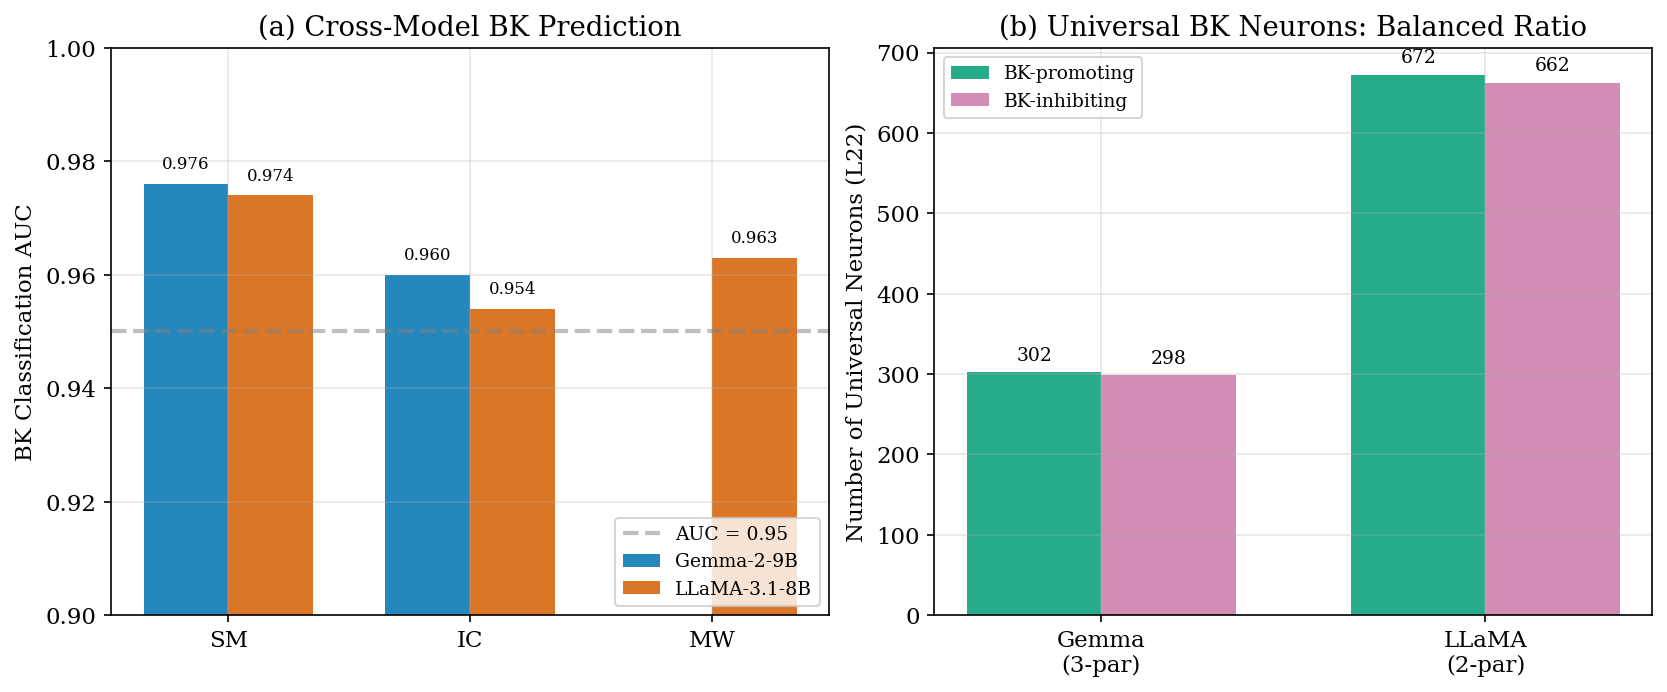
\includegraphics[width=\textwidth]{figures/v10_fig1_cross_model_bk.png}
\caption{(a) 교차 모델 BK 분류 AUC. (b) 보편적 BK 뉴런: 균형 잡힌 촉진/억제 비율.}
\label{fig:fig1}
\end{figure}

\noindent\textbf{그림~\ref{fig:fig1} 해석}: 패널 (a)는 Gemma와 LLaMA가 서로 다른 아키텍처와 훈련 데이터에도 불구하고 거의 동일한 BK 예측 정확도(모든 패러다임에서 AUC 차이 $< 0.02$)를 달성함을 보여준다. 패널 (b)는 두 모델 모두 거의 동일한 수의 촉진 뉴런과 억제 뉴런을 통해 BK를 인코딩함을 드러내며, 이는 일방적 위험 감지기가 아닌 양방향 ``push-pull'' 메커니즘을 시사한다.

\subsection{요인 분해}

요인 분해(Factor decomposition)는 배팅 유형과 패러다임을 통제한 후 SAE 피처 활성화에 대한 BK 결과의 독립적 기여를 분리한다. 각 피처에 대해 피처별 OLS 회귀(\texttt{feature $\sim$ outcome + bet\_type + paradigm})를 수행하여, 다른 요인을 편향시킨 후에도 결과가 유의($p<0.01$)한 피처를 식별한다.

\begin{table}[H]
\centering
\caption{요인 분해: 결과-유의 피처}\label{tab:t6}
\footnotesize
\begin{tabular}{lcccc}
\toprule
Model & Paradigms & Features Tested & Outcome-Significant (\%) & Permutation Null \\
\midrule
Gemma & IC+SM+MW (3-par) & 581 & \textbf{65.2\%} (379) & $\sim$1\% \\
LLaMA & IC+SM (2-par) & 1,418 & \textbf{69.5\%} (985) & $\sim$1\% \\
\textbf{LLaMA} & \textbf{IC+SM+MW (3-par)} & \textbf{1,056} & \textbf{75.8\%} (800) & $\sim$1\% \\
\bottomrule
\end{tabular}
\end{table}

\noindent LLaMA 3-패러다임 요인 분해(V10 신규)는 1,056개 피처 중 75.8\%가 배팅 유형 및 패러다임과 독립적으로 BK를 인코딩함을 보여주며, 이는 관찰된 최고 비율이다. 이 비율은 Gemma 3-패러다임(65.2\%)에서 LLaMA 2-패러다임(69.5\%)으로, 다시 LLaMA 3-패러다임(75.8\%)으로 증가한다. 세 번째 패러다임을 추가해도 BK 신호가 희석되지 않으며, 오히려 패러다임 특이적 노이즈를 필터링하여 신호가 집중된다.

\medskip\noindent 세 가지 분해 모두 약 1\%의 귀무 분포에 대해 순열 $p=0.000$을 산출하며, BK 표상 독립성이 통계적 인공물(artifact)이 아님을 확인한다.

\subsection{RQ1 종합}

BK 피처는 세 가지 독립적인 증거 라인에 의해 뒷받침되어 아키텍처 전반에 걸쳐 보편적이다. 첫째, BK 예측 정확도가 모델 간 거의 동일하다: SM에서 Gemma $0.976$ 대 LLaMA $0.974$이며, 두 모델 모두 IC와 MW에서 $0.95$를 초과한다. 둘째, 보편적 BK 뉴런이 두 모델 모두에서 균형 잡힌 촉진/억제 비율을 유지한다 (Gemma 302/298; LLaMA 672/662, L22). 이는 BK가 단방향 위험 감지기가 아닌 양방향 신호임을 나타낸다. 셋째, 요인 분해는 두 아키텍처 모두에서 SAE 피처의 65--76\%가 배팅 유형 및 패러다임과 독립적으로 BK를 인코딩함을 확인한다 (순열 $p=0.000$).

\medskip\noindent 이러한 발견은 BK 표상이 테스트된 두 트랜스포머 아키텍처의 공유 속성이며, 특정 단일 모델의 학습에 의한 인공물이 아님을 확립한다.

\bigskip\hrule\bigskip

% ============================================================
% 3. RQ2
% ============================================================
\section{RQ2: 도메인 불변성}

\noindent\textbf{연구 질문}: BK 패턴은 도박 도메인(IC, SM, MW) 간에 불변적인가?

\subsection{교차 도메인 전이}

교차 도메인 전이(Cross-domain transfer)는 한 패러다임의 피처로 BK 분류기를 훈련하고 다른 패러다임의 데이터에서 테스트한다. 전이 AUC가 우연 수준($0.5$)을 초과하고 순열 $p<0.05$이면, 두 패러다임은 BK 예측 구조를 공유한다.

\begin{table}[H]
\centering
\caption{Gemma SAE 교차 도메인 전이 (방향별 최적 층)}\label{tab:t7}
\footnotesize
\begin{tabular}{lccc}
\toprule
Transfer & Best Layer & AUC & perm\_$p$ \\
\midrule
IC $\rightarrow$ SM & L26 & \textbf{0.913} & 0.000 \\
IC $\rightarrow$ MW & L18 & \textbf{0.932} & 0.000 \\
SM $\rightarrow$ MW & L30 & \textbf{0.867} & 0.000 \\
SM $\rightarrow$ IC & L30 & 0.646 & 0.000 \\
MW $\rightarrow$ IC & L22 & 0.853 & 0.000 \\
\bottomrule
\end{tabular}
\end{table}

\begin{table}[H]
\centering
\caption{LLaMA 3-패러다임 은닉 상태 교차 도메인 전이 (V10 신규)}\label{tab:t8}
\footnotesize
\begin{tabular}{lccc}
\toprule
Transfer & Best Layer & AUC & $p$ \\
\midrule
\textbf{MW $\rightarrow$ IC} & \textbf{L25} & \textbf{0.805} & \textbf{0.000} \\
MW $\rightarrow$ IC & L12 & 0.797 & 0.000 \\
MW $\rightarrow$ IC & L22 & 0.724 & 0.000 \\
IC $\rightarrow$ MW & L8 & 0.680 & 0.000 \\
IC $\rightarrow$ MW & L25 & 0.587 & --- \\
SM $\rightarrow$ IC & L30 & 0.749 & 0.000 \\
SM $\rightarrow$ IC & L25 & 0.679 & --- \\
SM $\rightarrow$ IC & L22 & 0.646 & --- \\
IC $\rightarrow$ SM & L8 & 0.577 & 0.000 \\
\bottomrule
\end{tabular}
\end{table}

\begin{table}[H]
\centering
\caption{LLaMA 2-패러다임 SAE 교차 도메인 전이 (V9 기준선)}\label{tab:t9}
\footnotesize
\begin{tabular}{lccc}
\toprule
Transfer & Best Layer & AUC & perm\_$p$ \\
\midrule
IC $\rightarrow$ SM & L25 & \textbf{0.783} & 0.000 \\
SM $\rightarrow$ IC & L30 & \textbf{0.685} & 0.000 \\
\bottomrule
\end{tabular}
\end{table}

\noindent LLaMA 3-패러다임 전이(V10)는 두 가지 패턴을 보여준다. 첫째, MW $\rightarrow$ IC가 가장 강한 전이 방향이며 (L25 AUC$=0.805$), MW와 IC가 상당한 BK 구조를 공유함을 나타낸다. 둘째, IC $\rightarrow$ SM은 두 모델 및 두 표상 유형(SAE와 은닉 상태) 모두에서 가장 약한 방향으로 남아 있어, IC와 SM이 부분적으로 구별되는 메커니즘을 통해 BK를 인코딩함을 확인한다.

\medskip\noindent 전이 비대칭성(Transfer asymmetry)은 모델 간에 일관적이다: Gemma와 LLaMA 모두 *-to-MW 및 MW-to-* 전이가 강하며, IC--SM 전이는 층에 따라 달라진다.

\begin{figure}[H]
\centering
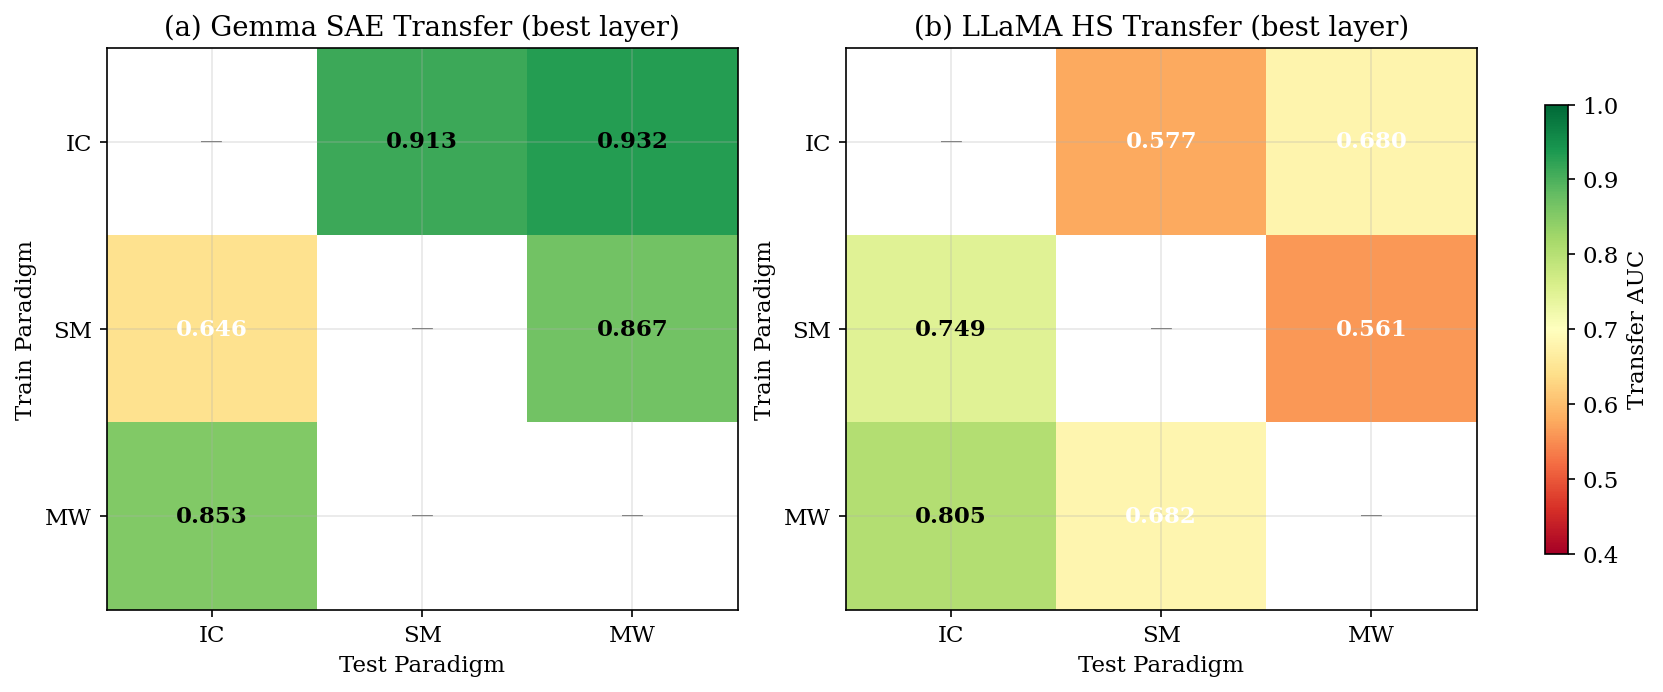
\includegraphics[width=\textwidth]{figures/v10_fig2_cross_domain_transfer.png}
\caption{교차 도메인 전이 AUC 히트맵. (a) Gemma SAE. (b) LLaMA 은닉 상태.}
\label{fig:fig2}
\end{figure}

\noindent\textbf{그림~\ref{fig:fig2} 해석}: 녹색 셀은 성공적 전이(AUC $\gg 0.5$)를, 적색 셀은 실패를 나타낸다. MW 패러다임은 두 모델 모두에서 강력한 ``허브'' 역할을 한다 --- MW에서 학습된 BK 패턴은 다른 도메인으로 잘 전이되며, 그 반대도 마찬가지이다. IC$\leftrightarrow$SM 전이는 일관되게 약하며, 이는 이 두 패러다임이 동일한 기본 결과를 공유함에도 불구하고 부분적으로 구별되는 메커니즘을 통해 BK를 인코딩함을 시사한다.

\subsection{공유 BK 부분공간}

패러다임별 LogReg 분류기는 서로 다른 방향을 가리키는 가중치 벡터를 생성한다 (코사인 $\approx 0.04$). 이 가중치 벡터에 대한 PCA는 저차원 공유 부분공간을 추출한다. 이 부분공간이 각 패러다임에 개별적으로 적용될 때 높은 AUC를 달성하면, BK 신호는 단일 축이 아닌 부분공간 전체에 분포되어 있는 것이다.

\begin{table}[H]
\centering
\caption{공유 BK 부분공간 성능}\label{tab:t10}
\footnotesize
\begin{tabular}{lcc}
\toprule
 & Gemma L22 (3D, 3-paradigm) & LLaMA L22 (2D, IC+SM) \\
\midrule
IC AUC & 0.862 $\pm$ 0.029 & \textbf{0.901} \\
SM AUC & 0.899 $\pm$ 0.034 & \textbf{0.943} \\
MW AUC & 0.970 $\pm$ 0.016 & --- \\
Weight cosines & IC--SM$=0.042$, IC--MW$=-0.026$, SM--MW$=-0.026$ & IC--SM$=\mathbf{0.038}$ \\
\bottomrule
\end{tabular}
\end{table}

\noindent LLaMA의 2D 공유 부분공간은 해당 패러다임에 대해 Gemma의 3D 부분공간($0.862$, $0.899$)보다 높은 AUC ($0.901$, $0.943$)를 달성한다. 두 모델 모두 동일한 구조적 속성을 공유한다: 가중치 벡터가 거의 직교(코사인 약 $0.04$)하지만, 저차원 부분공간이 AUC $> 0.86$으로 BK 신호를 포착한다. BK 신호는 단일 방향에 집중되지 않고 부분공간 전체에 분포되어 있다.

\subsection{은닉 상태 전이가 SAE 전이를 초과}

BK 신호가 다수의 뉴런에 분포되어 있다면, 모든 차원을 보존하는 은닉 상태 전이가 개별 피처로 희소화하는 SAE 전이보다 우수해야 한다.

\begin{table}[H]
\centering
\caption{은닉 상태 대 SAE 전이 (Gemma L22)}\label{tab:t11}
\footnotesize
\begin{tabular}{lccc}
\toprule
Transfer & Hidden AUC & SAE AUC & Delta \\
\midrule
IC $\rightarrow$ SM & \textbf{0.746} & 0.499 (NS) & $+0.247$ \\
IC $\rightarrow$ MW & \textbf{0.826} & 0.876 & $-0.050$ \\
SM $\rightarrow$ MW & \textbf{0.920} & 0.819 & $+0.101$ \\
\bottomrule
\end{tabular}
\end{table}

\begin{table}[H]
\centering
\caption{LLaMA 은닉 상태 대 SAE 전이 (IC $\leftrightarrow$ SM)}\label{tab:t12}
\footnotesize
\begin{tabular}{lccc}
\toprule
Transfer & Hidden AUC (best layer) & SAE AUC (best layer) & HS advantage \\
\midrule
SM $\rightarrow$ IC & 0.749 (L30) & 0.685 (L30) & $+0.064$ \\
IC $\rightarrow$ SM & 0.577 (L8) & 0.783 (L25) & $-0.206$ \\
\bottomrule
\end{tabular}
\end{table}

\noindent 은닉 상태는 대부분의 전이 방향에서 SAE를 능가한다 (Gemma IC$\rightarrow$SM $+0.247$; Gemma SM$\rightarrow$MW $+0.101$; LLaMA SM$\rightarrow$IC $+0.064$). 예외는 LLaMA IC$\rightarrow$SM으로, L25의 SAE ($0.783$)가 L8의 은닉 상태 ($0.577$)를 초과하지만, 이들은 서로 다른 층이다. 일반적인 패턴은 BK 신호가 희소적이지 않고 분포되어 있음을 확인한다: SAE 희소화는 교차 도메인 전이에서 일관성을 잃을 수 있다.

\subsection{RQ2 종합}

교차 도메인 불변성은 네 가지 수렴하는 분석에 의해 뒷받침된다:

\begin{table}[H]
\centering
\caption*{\textbf{RQ2 증거 요약}}
\footnotesize
\begin{tabular}{llp{7cm}}
\toprule
Evidence & Strength & Key Number \\
\midrule
Gemma IC$\rightarrow$MW transfer & \textbf{Strong} & AUC $0.932$ (L18, $p=0.000$) \\
LLaMA MW$\rightarrow$IC transfer (V10 NEW) & \textbf{Strong} & AUC $0.805$ (L25, $p=0.000$) \\
Gemma SM$\rightarrow$MW transfer & \textbf{Strong} & AUC $0.867$ (L30, $p=0.000$) \\
Factor decomposition (3-paradigm) & \textbf{Strong} & 65.2\% (Gemma), 75.8\% (LLaMA) \\
Shared BK subspace (both models) & \textbf{Strong} & AUC $0.86$--$0.97$, orthogonal weights \\
Gemma 3-paradigm SAE consistency (L18+) & \textbf{Strong} & 33--45\% vs 25\% chance, $p<5\times10^{-3}$ \\
LLaMA IC$\rightarrow$SM transfer & \textbf{Moderate} & SAE L25$=0.783$ only \\
LLaMA IC$\rightarrow$SM hidden state & \textbf{Weak} & L8$=0.577$ only; rest NS \\
\bottomrule
\end{tabular}
\end{table}

\noindent V10은 LLaMA에 MW 차원을 추가하여 RQ2를 진전시키며, MW$\rightarrow$IC가 LLaMA에서 가장 강한 3-패러다임 전이 방향(AUC $0.805$)임을 입증한다. 도메인 불변성은 표면적 구조가 더 많이 다른 패러다임 간에 가장 강하며 (MW 대 IC), 이는 표면 수준의 과제 특성이 달라질 때 BK 표상이 더 추상적이고 전이 가능해짐을 시사한다.

\bigskip\hrule\bigskip

% ============================================================
% 4. RQ3
% ============================================================
\section{RQ3: 프롬프트 조건 효과}

\noindent\textbf{연구 질문}: BK 패턴은 프롬프트 조건(고정/변동 배팅 유형, G/M/W/P/H 프롬프트 구성 요소) 간에 불변적인가?

\subsection{교차 배팅 유형 BK 전이 (F1)}

V10의 가장 중요한 발견은 한 배팅 유형에서 훈련된 BK 분류기가 다른 유형으로 전이된다는 직접적 입증이다. 코사인 유사도(cosine similarity)나 공유 뉴런 비율(V9)과 달리, 이 분석은 기능적 동등성(functional equivalence)을 테스트한다: 고정(Fixed)으로 훈련된 모델이 변동(Variable) BK를 예측할 수 있는가, 그리고 그 반대도 가능한가?

\begin{table}[H]
\centering
\caption{LLaMA IC 은닉 상태 교차 배팅 유형 전이}\label{tab:t13}
\footnotesize
\begin{tabular}{lcccc}
\toprule
Layer & Fix $\rightarrow$ Var AUC & $p$ & Var $\rightarrow$ Fix AUC & $p$ \\
\midrule
L8 & \textbf{0.872} & 0.000 & \textbf{0.842} & 0.000 \\
L12 & 0.772 & 0.000 & \textbf{0.927} & 0.000 \\
L22 & 0.736 & 0.000 & \textbf{0.912} & 0.000 \\
L30 & 0.819 & 0.000 & \textbf{0.911} & 0.000 \\
\bottomrule
\end{tabular}
\end{table}

\noindent\textbf{모든 방향, 모든 층: $p=0.000$.} 가장 약한 전이(Fix$\rightarrow$Var L22: $0.736$)조차 우연 수준을 상당히 초과한다. Var$\rightarrow$Fix 전이가 일관되게 더 강하며 ($0.842$--$0.927$), 이는 변동(Variable) BK 게임이 고정(Fixed) BK 영역을 포괄하는 더 넓은 활성화 공간을 탐색하기 때문일 수 있다.

\begin{table}[H]
\centering
\caption{Gemma IC SAE 교차 배팅 유형 전이}\label{tab:t14}
\footnotesize
\begin{tabular}{lcccc}
\toprule
Layer & Fix $\rightarrow$ Var AUC & $p$ & Var $\rightarrow$ Fix AUC & $p$ \\
\midrule
L18 & \textbf{0.808} & 0.000 & \textbf{0.726} & 0.000 \\
L30 & \textbf{0.902} & 0.000 & \textbf{0.696} & 0.000 \\
L10 & NS & --- & NS & --- \\
\bottomrule
\end{tabular}
\end{table}

\noindent Gemma는 반대 비대칭성을 보인다: Fix$\rightarrow$Var ($0.808$--$0.902$)가 Var$\rightarrow$Fix ($0.696$--$0.726$)를 초과한다. 얕은 층(L10)은 실패하며, 이는 교차 도메인 및 교차 조건 전이에 깊은 층의 표상이 필요하다는 일반적 발견과 일치한다.

\medskip\noindent\textbf{종합}: 교차 배팅 유형 전이는 두 모델 모두에서 깊은 층에서 성공한다 (AUC $0.696$--$0.927$, 모두 $p=0.000$). BK 표상은 고정/변동 조작에 대해 불변적이다. 이는 지금까지의 가장 강력한 RQ3 증거이다: 단순히 공유 방향(코사인)이나 공유 뉴런(상호작용 회귀)이 아닌, 성공적인 분류 전이를 입증한다.

\begin{figure}[H]
\centering
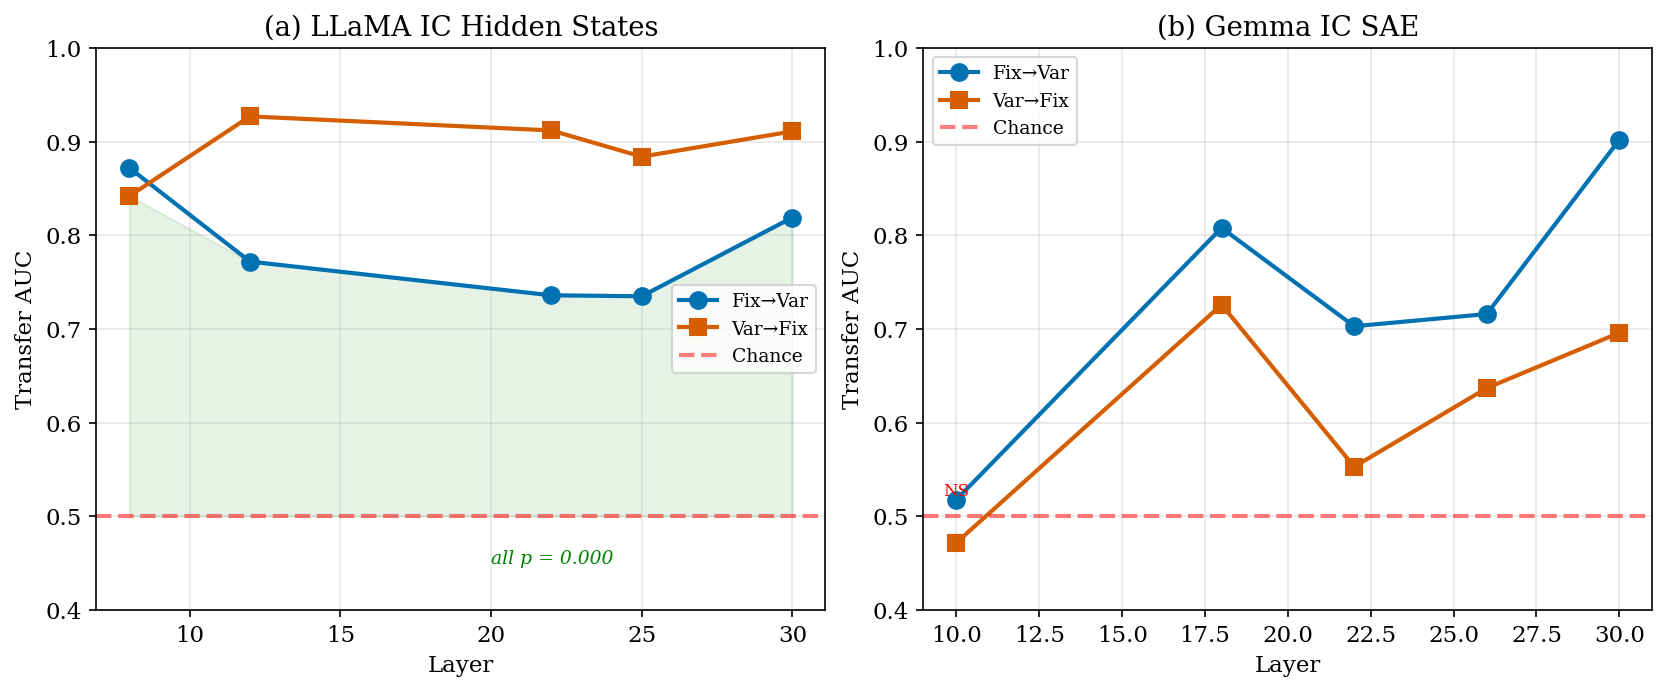
\includegraphics[width=\textwidth]{figures/v10_fig3_cross_bettype_transfer.png}
\caption{교차 배팅 유형 BK 전이. (a) LLaMA HS: 모든 층 $p=0.000$. (b) Gemma SAE: 깊은 층에서 성공.}
\label{fig:fig3}
\end{figure}

\noindent\textbf{그림~\ref{fig:fig3} 해석}: 이것이 V10의 핵심 발견이다. 고정 배팅 파산 게임만으로 훈련된 BK 분류기가 변동 배팅 파산을 AUC $0.872$ (LLaMA L8)까지 예측할 수 있으며, 그 반대 방향도 $0.927$ (L12)에 도달한다. 녹색 음영 영역은 우연 수준($0.5$) 위의 격차를 보여주며 --- 모든 점이 이를 크게 초과한다. 이는 변동 배팅이 더 높은 행동적 파산율을 유발함에도 불구하고, 고정 및 변동 배팅이 동일한 기본 BK 표상을 활성화함을 입증한다.

\subsection{배팅 유형 간 공통 BK 피처}

공통 BK 피처(Common BK feature)는 고정 및 변동 조건 모두에서 BK 게임과 안전 게임 간 Cohen's $d \ge 0.3$이며, 동일한 부호를 가지는 피처로 정의된다. 이 피처들은 배팅 자율성에 관계없이 BK를 인코딩한다.

\begin{table}[H]
\centering
\caption{변동/고정 공통 BK 피처 (LLaMA IC SAE L22)}\label{tab:t15}
\footnotesize
\begin{tabular}{lc}
\toprule
Criterion & Count \\
\midrule
Total features with $d \ge 0.3$ in BOTH bet types (same sign) & \textbf{415} \\
BK-promoting & 213 \\
BK-inhibiting & 202 \\
\bottomrule
\end{tabular}
\end{table}

\noindent 415개의 공통 피처(촉진 213 / 억제 202)는 보편적 BK 뉴런(2.2절)에서 관찰된 균형 비율을 유지한다. 이 피처들은 모델이 고정 또는 변동 배팅 자율성을 가지는지에 관계없이 BK를 인코딩한다. 균형 잡힌 촉진/억제 구조는 피처 수준에서 보존되어, BK 표상의 양방향적 특성을 강화한다.

\subsection{G-프롬프트 BK 방향 정렬}

G-프롬프트 방향(G-prompt direction)은 G-존재 게임과 G-부재 게임 간의 평균 은닉 상태 차이로 정의된다. BK 방향은 BK 게임과 안전 게임 간의 평균 차이이다. 이 두 벡터 간의 양의 코사인은 G가 활성화 공간을 파산 방향으로 이동시킴을 나타낸다.

\begin{table}[H]
\centering
\caption{G-프롬프트 BK 방향 정렬 (교차 모델)}\label{tab:t16}
\footnotesize
\begin{tabular}{lcc}
\toprule
 & Gemma SM & LLaMA SM \\
\midrule
BK with G & 5.2\% & 40.6\% \\
BK without G & 0.3\% & 32.2\% \\
Ratio & \textbf{20.75$\times$} & \textbf{1.26$\times$} \\
$\cos(G_\mathrm{dir}, BK_\mathrm{dir})$ L22 & $\mathbf{+0.850}$ & $\mathbf{+0.634}$ \\
$\cos(G_\mathrm{dir}, BK_\mathrm{dir})$ L30 & --- & $\mathbf{+0.548}$ \\
\bottomrule
\end{tabular}
\end{table}

\noindent 두 모델 모두 L22에서 G-프롬프트 방향과 BK 방향 간에 양의 코사인을 보인다 (Gemma $+0.850$; LLaMA $+0.634$). G는 두 아키텍처 모두에서 활성화를 BK 영역으로 밀어낸다. 행동적 효과 크기 차이($20.75\times$ 대 $1.26\times$)는 질적 메커니즘 차이를 반영하지 않는다; 오히려, Gemma의 BK 기저율이 극히 낮아(0.3\%) 적은 방향적 이동도 큰 비율 변화를 유발한다.

\medskip\noindent LLaMA L30 코사인 ($+0.548$)은 깊은 층에서도 정렬이 지속됨을 확인하며, BK 표상의 깊이 불변적 특성과 일치한다.

\subsection{배팅 제한 선형 매핑}

IC는 네 가지 배팅 제한(c10, c30, c50, c70)을 사용하여 최대 배팅을 \$10--\$70으로 제한한다. 높은 상한은 라운드당 더 큰 손실을 허용하여 객관적 BK 위험을 증가시킨다. 모델의 내부 BK 확률이 제한 수준에 따라 선형적으로 스케일링된다면, BK 표상은 단순한 이진 BK/Safe 구분이 아닌 연속적 위험 크기를 인코딩하는 것이다.

\begin{table}[H]
\centering
\caption{배팅 제한 $\rightarrow$ BK 확률 (교차 모델, IC SAE L22)}\label{tab:t17}
\footnotesize
\begin{tabular}{ccccc}
\toprule
Constraint & Gemma BK prob & LLaMA BK prob & Gemma Actual BK\% & LLaMA Actual BK\% \\
\midrule
c10 & 0.000 & 0.057 & 0.0\% & --- \\
c30 & 0.056 & 0.113 & 5.2\% & --- \\
c50 & 0.212 & 0.233 & 16.8\% & --- \\
c70 & 0.270 & 0.360 & 21.0\% & --- \\
\bottomrule
\end{tabular}

\medskip
\begin{tabular}{lcc}
\toprule
 & Gemma & LLaMA \\
\midrule
Linear $r$ & \textbf{0.979} & \textbf{0.987} \\
$p$ & 0.021 & 0.013 \\
\bottomrule
\end{tabular}
\end{table}

\noindent 두 모델 모두 거의 완벽한 선형 관계를 보인다 ($r > 0.97$, $p < 0.025$). BK 표상은 객관적 위험 노출(배팅 상한)에 따라 연속적으로 스케일링된다. LLaMA의 약간 더 높은 $r$ ($0.987$ 대 $0.979$)과 더 가파른 기울기(c10: $0.057$에서 c70: $0.360$)는 더 민감한 위험 스케일링 메커니즘을 나타낸다.

\begin{figure}[H]
\centering
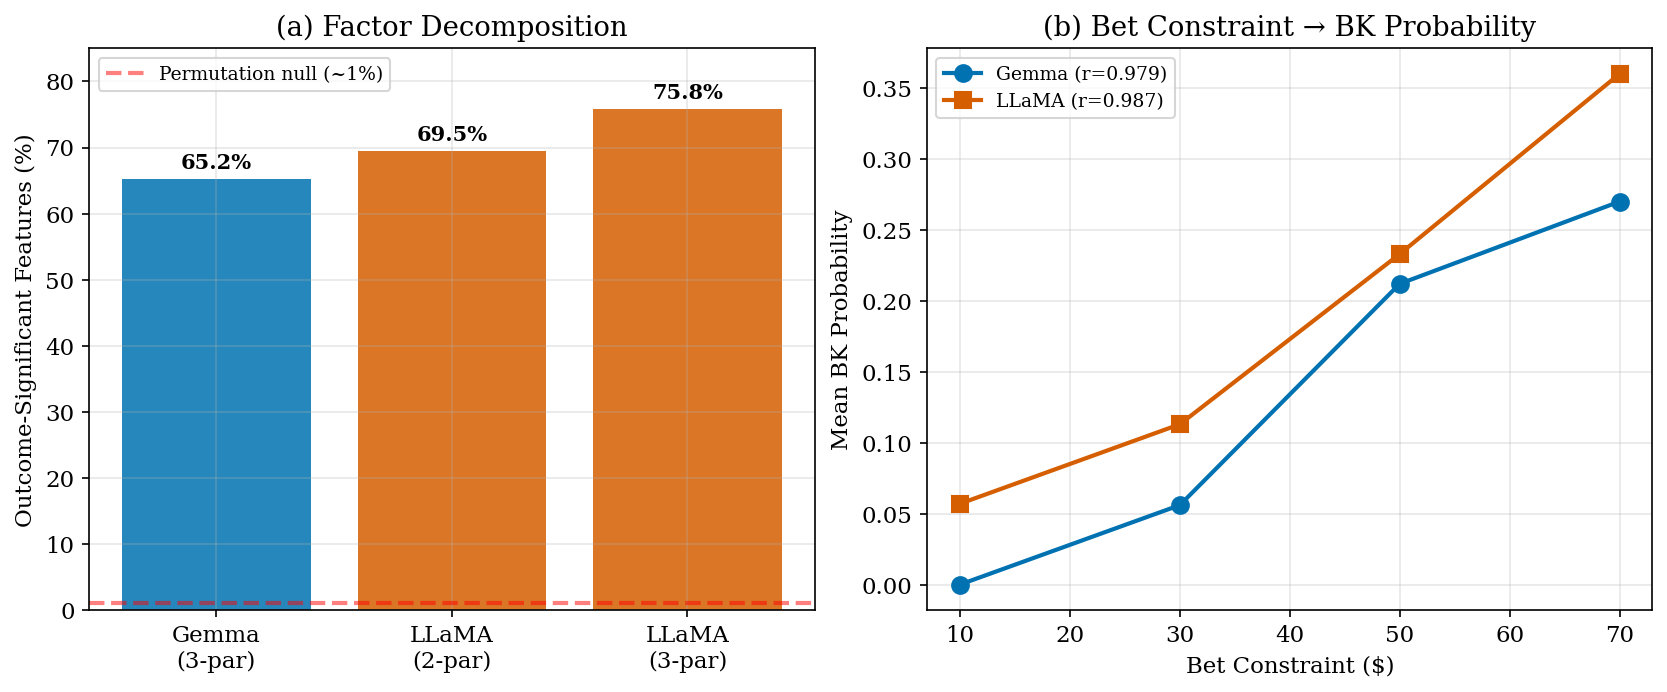
\includegraphics[width=\textwidth]{figures/v10_fig4_factor_constraint.png}
\caption{(a) 요인 분해: 결과-유의 65--76\% 대 귀무 1\%. (b) 배팅 제한 선형 매핑.}
\label{fig:fig4}
\end{figure}

\noindent\textbf{그림~\ref{fig:fig4} 해석}: 패널 (a)는 BK를 인코딩하는 SAE 피처의 대다수가 교란 변수와 독립적으로 인코딩함을 보여준다. 1\%의 적색 점선은 순열 귀무 분포를 나타내며 --- 실제 비율(65--76\%)은 이를 $60\times$+ 초과한다. 패널 (b)는 배팅 제한이 \$10에서 \$70으로 증가함에 따라 모델의 내부 BK 확률이 선형적으로 증가함을 입증하며, BK 표상이 이진 안전/불안전 구분이 아닌 연속적 위험 크기를 인코딩함을 확인한다.

\subsection{RQ3 종합}

네 가지 분석이 조건 불변적 BK 표상을 확립한다:

\begin{table}[H]
\centering
\caption*{\textbf{RQ3 증거 요약}}
\footnotesize
\begin{tabular}{llp{7cm}}
\toprule
Evidence & Strength & Key Number \\
\midrule
\textbf{Cross-bet-type transfer F1 (V10 NEW)} & \textbf{Strong} & AUC $0.736$--$0.927$, all $p=0.000$ (both models) \\
Common BK features across bet types (V10 NEW) & \textbf{Strong} & 415 features, balanced 213/202 \\
LLaMA IC Var/Fix cosine $> 0.81$ & \textbf{Strong} & All 5 layers, balanced sample \\
Shared BK neurons $\sim$33--37\% (IC) & \textbf{Strong} & Cross-model consistent \\
G-prompt BK alignment (both models) & \textbf{Strong} & $\cos$ $+0.634$ to $+0.850$ at L22 \\
Bet constraint linear mapping & \textbf{Strong} & $r = 0.979$ (Gemma), $0.987$ (LLaMA) \\
Balance confound control & \textbf{Strong} & 99.7--101\% retained \\
\bottomrule
\end{tabular}
\end{table}

\noindent V10은 F1 교차 배팅 유형 전이 분석을 통해 RQ3를 결정적으로 진전시킨다. V9는 간접적 증거(코사인 유사도, 공유 뉴런 비율)를 제공했고, V10은 직접적 증거(성공적 분류 전이)를 제공한다. 고정 배팅 BK 게임만으로 훈련된 분류기가 변동 배팅 BK 게임을 AUC $0.927$까지 예측할 수 있으며 (반대 방향도 마찬가지), 이는 BK 표상이 배팅 자율성에 대해 기능적으로 불변적임을 입증한다.

\bigskip\hrule\bigskip

% ============================================================
% 5. IMPLICATIONS
% ============================================================
\section{NMT 논문 3.2절에 대한 시사점}

논문의 3.2절은 활성화 패칭(Activation patching)을 통해 LLaMA SM에서 112개의 인과적 피처(causal features)를 식별하였으며, 안전 피처는 L4--L19에 집중되고 위험 피처는 L24+에 집중된다. 이 피처들은 양방향 인과 효과와 목표 추구 대 중단 어휘와의 의미적 연관을 보인다. V10은 이 단일 모델, 단일 도메인 발견을 세 방향으로 확장한다.

\medskip\noindent\textbf{1. 교차 모델 검증.} 112개의 인과적 피처는 LLaMA SM에서 식별되었다. V10은 Gemma가 거의 동일한 BK 분류($0.976$ 대 $0.974$), 균형 잡힌 촉진/억제 구조를 가진 600개의 보편적 BK 뉴런, 65.2\%의 결과-독립적 피처를 달성함을 보여준다. 이는 인과적 피처가 LLaMA 특이적 인공물이 아니라 두 아키텍처가 공유하는 속성을 반영함을 확립한다.

\medskip\noindent\textbf{2. 교차 도메인 일반화.} 인과적 피처는 슬롯머신 패러다임에서 식별되었다. V10의 교차 도메인 전이 (Gemma IC$\rightarrow$MW AUC $0.932$; LLaMA MW$\rightarrow$IC AUC $0.805$)와 요인 분해(65--76\% 패러다임 독립적)는 BK 표상이 특정 도박 도메인을 넘어 일반화됨을 입증한다. BK의 신경적 기반은 과제 특이적 패턴 매칭이 아닌, 도메인 일반적 위험 계산(domain-general risk computation)을 반영한다.

\medskip\noindent\textbf{3. 교차 조건 견고성.} F1 교차 배팅 유형 전이 (AUC $0.736$--$0.927$, 모두 $p=0.000$)는 BK 표상이 고정/변동 자율성 조작에 대해 견고함을 입증한다. 선형 배팅 제한 매핑($r > 0.97$)과 결합하면, 인과적 피처가 위험 노출에 따라 연속적으로 스케일링되고 표면적 과제 매개변수에 불변적인 표상 공간 내에서 작동함을 보여준다.

\medskip\noindent 이 세 가지 확장은 3.2절을 단일 모델, 단일 도메인 인과 분석에서 다중 모델, 다중 도메인, 다중 조건 메커니즘적 설명으로 변환한다.

\bigskip\hrule\bigskip

% ============================================================
% 6. LIMITATIONS
% ============================================================
\section{한계점}

\subsection{BK 비율 이질성}

\begin{table}[H]
\centering
\footnotesize
\begin{tabular}{lcccccc}
\toprule
 & Gemma IC & LLaMA IC & Gemma SM & LLaMA SM & Gemma MW & LLaMA MW \\
\midrule
BK\% & 10.8\% & 8.9\% & 2.7\% & 36.4\% & 1.7\% & 75.8\% \\
\bottomrule
\end{tabular}
\end{table}

\noindent LLaMA MW BK 비율(75.8\%)은 Gemma MW(1.7\%)의 $44\times$이다. 행동 수준에서의 교차 모델 비교는 이러한 기저 비율 차이에 의해 교란된다. 분류 AUC(균형 클래스 가중치 사용)는 이를 부분적으로 완화하지만, 저-BK 조건에서의 소표본 팽창으로 인해 모델 간 효과 크기(Cohen's $d$) 비교는 여전히 신뢰할 수 없다.

\subsection{상관적 증거}

본 보고서의 모든 분석은 상관적이다. 논문의 112개 인과적 피처는 활성화 패칭(LLaMA SM에서만)에서 비롯된다. 교차 모델 및 교차 도메인 인과 검증(Gemma 활성화 패칭, IC/MW 패칭)은 보류 중이다. 전이 AUC는 공유 표상을 입증하지만 인과적 필요성(causal necessity)을 확립하지는 않는다.

\subsection{통계적 검정력 불균형}

\begin{table}[H]
\centering
\footnotesize
\begin{tabular}{lp{9cm}}
\toprule
Analysis & Weakness \\
\midrule
Gemma IC Variable BK & $n=14$ (배팅 유형 비교에 대한 매우 낮은 검정력) \\
Gemma MW BK & $n=54$ (MW 특이적 분석 제한) \\
LLaMA 2-paradigm sign-consistency & 50\% 우연 수준; 이항 검정에서 13/16 층이 NS \\
\bottomrule
\end{tabular}
\end{table}

\subsection{LLaMA 은닉 상태 층 커버리지}

LLaMA 은닉 상태는 5개 층(L8, L12, L22, L25, L30)에서만 추출되며, 전체 32개 층에서 추출되지 않는다. 이 체크포인트 사이의 층 특이적 현상이 누락될 수 있다. Gemma는 더 넓은 층 커버리지를 가진다.

\subsection{다중 비교 문제}

FDR 보정은 개별 분석(예: 보편적 뉴런 식별) 내에서 적용되지만, 전체 분석 집합에 걸쳐서는 적용되지 않는다. 모델, 층, 패러다임에 걸친 뉴런별 및 피처별 검정은 큰 총 검정 수를 생성한다. 효과 크기를 일차 증거로, $p$-값을 이차 증거로 취급해야 한다.

\bigskip\hrule\bigskip

% ============================================================
% 7. NEXT STEPS
% ============================================================
\section{향후 과제}

\begin{enumerate}[nosep]
    \item \textbf{Gemma 활성화 패칭}: Gemma의 600개 보편적 BK 뉴런과 상위 교차 도메인 피처가 BK 결과에 인과적으로 필요한지 검증. 교차 모델 인과 검증을 위한 핵심 실험.
    \item \textbf{IC/MW 활성화 패칭}: SM에서 식별된 인과적 피처의 IC 및 MW에서의 인과 효과 테스트, 교차 도메인 인과 일반화를 직접 검증.
    \item \textbf{Gemma 교차 배팅 유형 전이 (은닉 상태)}: SAE뿐만 아니라 Gemma 은닉 상태를 사용한 F1 분석 복제, 교차 배팅 유형 불변성의 모델 일반적 특성 확인.
    \item \textbf{G-프롬프트 메커니즘 심층 분석}: G가 Gemma에서 $20.75\times$ BK 효과를 생성하지만 LLaMA에서는 $1.26\times$만 생성하는 이유 조사. 코사인 정렬 차이($0.850$ 대 $0.634$)만으로는 $16\times$의 행동적 격차를 설명하지 못함.
    \item \textbf{LLaMA 3-패러다임 SAE 교차 도메인 일관성}: Gemma 7-층 부호 일관성 분석(V9 Table~5)을 IC+SM+MW를 사용한 LLaMA로 확장, 25\% 3-패러다임 우연 수준에 대한 검정.
\end{enumerate}

% ============================================================
% APPENDIX
% ============================================================
\appendix
\section{V9에서 V10으로의 주요 추가 사항 요약}

\begin{table}[H]
\centering
\caption{V9에서 V10으로의 추가 사항}\label{tab:a1}
\footnotesize
\begin{tabular}{lp{4cm}p{6cm}}
\toprule
Analysis & V9 Status & V10 Addition \\
\midrule
LLaMA MW data & Missing & \textbf{3,200 games, BK$=2{,}426$ (75.8\%)} \\
LLaMA MW classification & N/A & \textbf{AUC $0.963$ (L16), $0.96$+ all layers} \\
LLaMA 3-paradigm transfer & N/A & \textbf{MW$\rightarrow$IC AUC $0.805$ (L25)} \\
LLaMA 3-paradigm factor decomp & 2-paradigm: 69.5\% & \textbf{3-paradigm: 75.8\%} \\
Cross-bet-type transfer (F1) & Not tested & \textbf{LLaMA: AUC $0.736$--$0.927$ (all $p=0.000$)} \\
Cross-bet-type transfer (F1) & Not tested & \textbf{Gemma SAE: AUC $0.696$--$0.902$ (deep layers)} \\
Common BK features (bet-type) & Not quantified & \textbf{415 features (213 promoting, 202 inhibiting)} \\
LLaMA 2D BK subspace & Not computed & \textbf{IC AUC$=0.901$, SM AUC$=0.943$} \\
LLaMA G-prompt alignment & Behavioral only ($1.26\times$) & \textbf{$\cos(G_\mathrm{dir}, BK_\mathrm{dir})$: L22$=+0.634$, L30$=+0.548$} \\
LLaMA bet constraint mapping & Not computed & \textbf{$r=0.987$, $p=0.013$} \\
\bottomrule
\end{tabular}
\end{table}

\end{document}
